\chapter{Ensayos y resultados experimentales}

\section{Introducción}

Una vez implementado el sistema de control diseñado en la placa de desarrollo Nexys 3, se realizan una serie de ensayos para verificar su correcto funcionamiento. Estos ensayos fueron realizados en forma progresiva, en un principio probando sólamente el generador PWM junto con el ADC en un esquema lazo abierto. Luego de ir confirmando el correcto funcionamiento, se fueron agregando más componentes para finalmente realizar un ensayo con el lazo cerrado de tensión.

\section{Pruebas a lazo abierto}

Las primeras pruebas realizadas a lazo abierto consistieron en la utilización del controlador PWM para las señales de los transistores del convertidor CC-CC. Luego, se implementó al controlador del conversor analógico-digital para permitir la variación del ciclo de trabajo mediante un potenciómetro, cuyo valor era filtrado por el filtro diseñado e implementado a \SI{1.5}{\kilo\hertz}.

\section{Pruebas a lazo cerrado}

\subsection{Lazo de control de corriente}

El primer ensayo a lazo cerrado consistió en el control de la corriente por el inductor del convertidor CC-CC. En este sistema fueron utilizados los componentes ya probados anteriormente: el controlador PWM; el controlador del ADC; y el filtro de corriente de \SI{1.5}{\kilo\hertz}. Para poder cerrar el lazo, se incorporaron dos nuevos elementos: la referencia, para poder establecer un valor en el cual la corriente se establezca; y el controlador PI, para poder calcular la acción de control que permita seguir a la referencia.

Como medida de seguridad, se implementaron llaves que permiten habilitar o deshabilitar el integrador del controlador. Además, este componente posee una saturación a su salida, para evitar el cálculo de un ciclo de trabajo mayor a 1 o 100\%; y el método anti-windup explicado anteriormente.

Realizando escalones de \SI{3}{\ampere} con este sistema de control, se obtuvieron los siguientes resultados de las Figuras \ref{escalones-lazo-corriente}.

\begin{figure}[hbt!]
    \centering
    \subfloat[Escalón negativo de \SI{3}{\ampere}.]{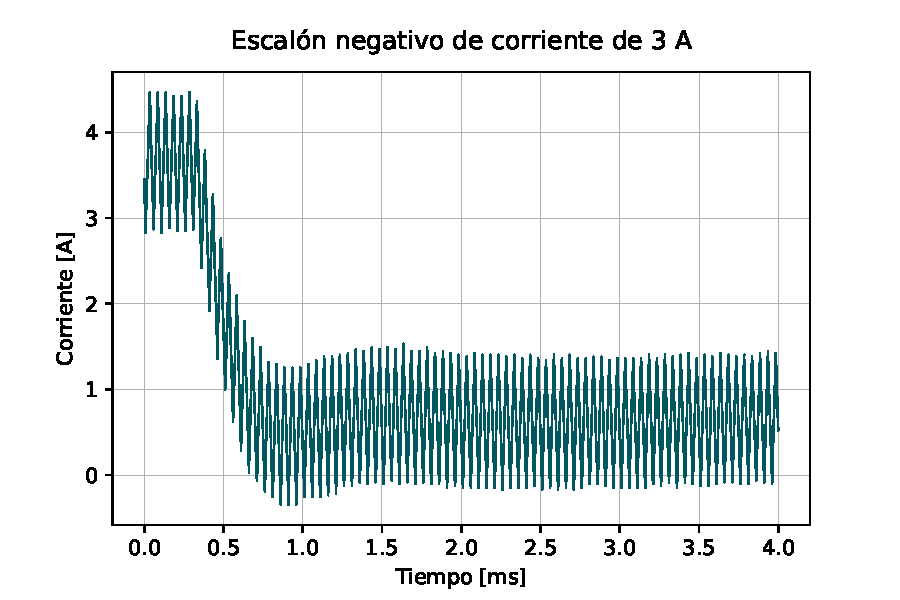
\includegraphics[width=0.45\textwidth]{Imágenes/Ensayos/Lazo interno de corriente/Fuente de potencia/Escalón negativo de corriente.pdf}}    
    \subfloat[Escalón positivo de \SI{3}{\ampere}.]{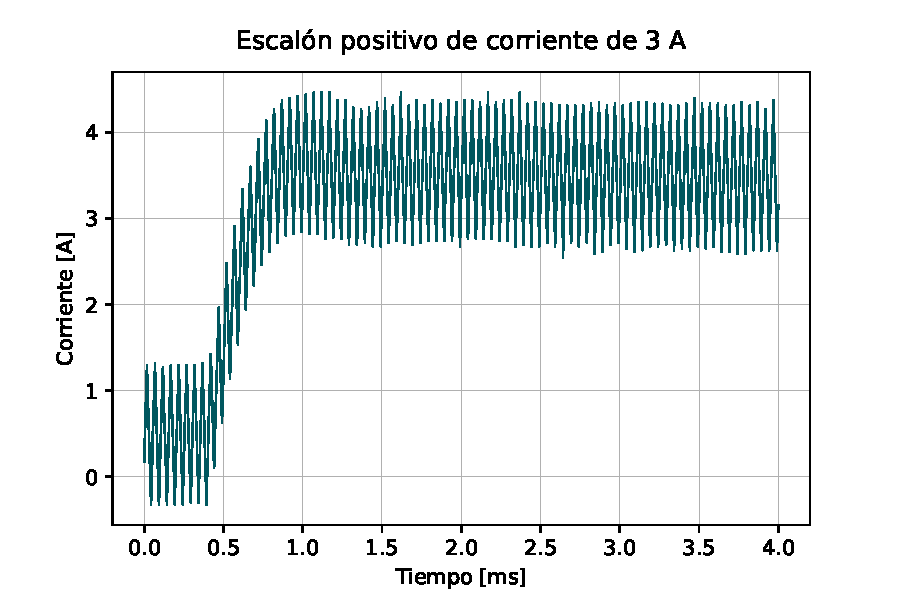
\includegraphics[width=0.45\textwidth]{Imágenes/Ensayos/Lazo interno de corriente/Fuente de potencia/Escalón positivo de corriente.pdf}}
    \caption{Resultados de los ensayos del lazo de corriente.}
    \label{escalones-lazo-corriente}

  \end{figure}



\newpage